\chapter{Norm\'al rendszerek, entr\'opia, intenz\'{\i}v param\'eterek, a statisztikus fizika \'es a termodinamika kapcsolata} 
 
 \paragraph{Állapotszám}
  
  Legyen egy $N$ részecskés kvantummechanikai rendszerünk. Ebben az energiaszintek: $E_i$. Az állapotszám:
  \al{
   \Omega_{0,\text{QM}}(E)=\frac{1}{N!}\suml{n}{}\Theta(E-E_n),
  }
  ami tehát összeszámolja, hogy hány energiaszint van $E$ alatt. Klasszikusan is hasonló a definíció:
  \al{
   \Omega_{0,\text{CL}}(E)=\intl{\substack{\text{állapotok,}\\ \text{ahol }E'<E}}{}\frac{\dd^{dN}p\dd^{dN}q}{N! h^{dN}}\,.
  }
  
 \paragraph{Differenciális állapotszám}
  
  Ez az az állapotszám, ami az $E$ és az $E+\delta E$ energia között található:
  \al{
   \Omega(E,\delta E)=\Omega_0(E+\delta E)-\Omega_0(E).
  }
  Itt $\delta E$ makroszkopikus energiakülönbségként van definiálva.
  
 \paragraph{Állapotsűrűség}
  
  Makroszkopikus rendszerben az energiaszintek nagyon sűrűn helyezkednek el, $N\to\infty$-ben folytonossá válnak. Ekkor a differenciális állapotszámban vehetjük a $\delta E\to\dd E\to 0$ határesetet. Ekkor:
  \al{
   &\Omega(E,\dd E)
    =\Omega_0(E+\dd E)-\Omega_0(E)
    =\der{\Omega_0(E)}{E}\dd E+\mathcal{O}(\dd E^2)
   &\omega(E)=\der{\Omega_0(E)}{E},
  }
  ahol $\omega(E)$ az állapotsűrűség. 
  
 \paragraph{Normál rendszerek}
  
  Normál rendszereknek nevezzük azokat a rendszereket, ahol 
  \aln{
   \ln\Omega_0(E)=N\phi\left(\frac{E}{N},\frac{V}{N}\right)+\mathcal{O}(\ln N),\label{eq:B03-Omega--N}
  }
  és $N\to\infty$-re $\frac{E}{N}$ és $\frac{V}{N}$ rögzített. Így tehát a részecskeszám növelésével az állapotszám exponenciálisan nő. 
  
  Léteznek nem normál rendszerek is, ott ez biztosan nem teljesül, ahol véges a rendszer véges állapottal rendelkezik. 
  
  Normál rendszerre egy példa az ideális gáz, a számolást klasszikus esetben lásd \aref{ss:B06-CID}.\ fejezetben. Nem normál rendszer bármilyen véges állapotú rendszer, például a spinrendszerek. Erre példa \aref{ss:neghom}.\ fejezetben. 
  
 \section{Mikrokanonikus sokaság ($E$,$V$,$N$)}\label{ss:B03-mikrokansok}
  
  A zárt rendszerhez tartozó sokaság a mikrokanonikus sokaság. Ekkor $E$, $N$ és $V$ rögzített. $E$-t nem tudjuk fizikailag sem rögzíteni, így abban megengedünk egy $\delta E$ makroszkopikus nagyságú bizonytalanságot, így azt állíthatjuk, hogy a rendszer energiája $E$ és $E+\delta E$ között van. 
  
  \subsection{Egyenlő valószínűségek elve}
   
   A rendszer állapotáról semmit nem tudunk, csak annyit, hogy az energiája a fenti sávban van. A statisztikus fizika egyik alapfeltevése az, hogy azt egyes állapotok valószínűsége ugyanakkora:
   \al{
    \rho(i)=\begin{cases}
             \frac{1}{\Omega(E,\delta E)}, & \text{ha } E_i\in [E,E+\delta E]\\
             0& \text{ egyébként.}
            \end{cases}
   }
   Ekkor tudunk a legkevesebbet a rendszerről.
   
  \subsection{Entrópia}
   
   A statisztikus fizikai entrópia definíció szerint:
   \al{
    S(E,V,N)=\kB\ln\Omega(E,\delta E),
   }
   ahol $\kB=1,38\cdot 10^{-23}\me{\frac{J}{K}}$ a Boltzmann-állandó. Kérdés, hogy mi köze ennek a termodinamikában definiált entrópiához. Ennek eldöntéséhez vizsgáljuk meg a statisztikus fizikai entrópia tulajdonságait:
   
   \begin{itemize} 
    \item
     Mivel az $\ln$ függvény monoton nő, ezért normál rendszeren $S$ akkor nő, ha $\Omega$ nő. Az állapotok számának növelésével a rendszer rendezetlensége, az, hogy milyen állapotban lehet a rendszer, nő, így az entrópia tekinthető a rendezetlenség mértékének.
    
    \item
     Spontán folyamatokban $S$ növekszik. Pl.\ ha egy gáz kezdetben el volt zárva, majd kinyitjuk a szelepet, és hagyjuk, hogy kitöltse a teret. Az entrópia nő, hiszen a tágulással a fázistér jóval megnőtt, így az állapotszám is megnövekedet.
     
    \item
     Izolált rendszerekben az entrópia additív. Legyen két izolált rendszerünk. Ezekben az állapotszám $\Omega_1(E_1,\delta E_1)$ és $\Omega_2(E_2,\delta E_2)$. A teljes rendszerben, mivel ezek függetlenek, a lehetséges állapotok száma ennek a kettőnek a szorzata, így 
     \al{
      S_{1+2}
      &=\kB\ln\Omega_{1+2}(E_1,\delta E_1;E_2,\delta E_2)
       =\kB\ln\big[\Omega_{1}(E_1,\delta E_1)\cdot \Omega_{2}(E_2,\delta E_2)\big]\\
      &=\kB\ln\Omega_{1}(E_1,\delta E_1)+\kB\ln\Omega_{2}(E_2,\delta E_2)
       =S_1+S_2.
     }
     
    \item
     $S$ definíció szerint megegyezik (egy szorzó erejéig) az információs entrópia maximumával:
     \al{
      S_\text{inf}
       &=-\suml{i}{}p_i\ln p_i
        =-\suml{i}{}\frac{1}{\Omega(E,\delta E)}\ln \frac{1}{\Omega(E,\delta E)}
        =-\ln \frac{1}{\Omega(E,\delta E)}\underbrace{\suml{i}{}\frac{1}{\Omega(E),\delta E)}}_{=1}\\
       &=\ln\Omega(E,\delta E)
        =\frac{1}{\kB}S.
     }
     
    \item
     Termodinamikai határesetben az állapotszám: $\Omega_0(E,\delta E)=\omega(E)\delta E$, így
     \al{
      S=\kB\ln\Omega(E,\delta E)
       =\kB\ln\big(\omega(E)\delta E)
       =\kB\ln\omega(E)+\kB\ln\delta E.
     } 
     Normál rendszerekben $\Omega\sim e^{N}$ így $\omega\sim e^{N}$ szintén, hiszen $E/N$ állandó. A $\delta E$ makroszkópikus nagyságú, vagyis nagyságrendileg $\sim E$, azaz $\sim N$. Innen tehát az adódik, hogy $S$ arányos egy $\sim N$ és egy $\sim\ln N$ taggal. A második tag elhagyható a termodinamikai határesetben, így: $S=\kB\ln\omega(E)$, $\delta E$-től függetlenül. 
     
     Az {\color{red} ÁBRÁ}ról látszik, hogy $\Omega(E,\delta E)<\Omega_0(E)<\omega(E)E$, melynek logaritmusát véve és kihasználva, hogy a termodinamikai határesetben $\ln E$ jóval elhagyható $\ln\omega(E)$ mellett, következik, hogy $S=\kB\Omega_0(E)$ is fennáll. Összefoglalva:
     \aln{
      S=\kB\ln\omega(E)=\kB\ln\Omega_0(E).\label{eq:B03-entropia}
     }
     
     Fontos, hogy az $S$ ilyen módon történő átírása csak normál rendszerekre lehetséges, a $\delta E$-től való függés csak ott küszöbölhető ki.
   \end{itemize}
   
  \subsection{Termikus kapcsolatban lévő alrendszerek, hőmérséklet}
   
   Legyen egy zárt rendszerünk, melyet két termikus kapcsolatban álló alrendszerre osztottunk. Rövidtávú kölcsönhatások esetén a kölcsönhatási energia elhanyagolható a két alrendszer között, így $E=E_1+E_2$. $E_1$ és $E_2$ változhat a kölcsönhatások miatt, egyedül annyit tudunk, hogy az egész rendszer zárt, így $E_1+E_2=E$ az $E$ és a $E+\delta E$ tartományon van. A kölcsönhatást csak abban az értelemben vesszük figyelembe, hogy ez termalizálja a két rendszert, de a rendszerek állapotának számításakor nem vesszük figyelembe.
   
   Írjuk fel a teljes rendszer állapotszámát, figyelembe véve azt, hogy a két rendszer állapotszáma független:
   \al{
    \Omega(E,\delta E)
     &=\intl{E_1+E_2\in[E,E+\delta E]}{}\dd E_1\dd E_2 \,\omega_1(E_1)\omega_2(E_2)
     \approx\intl{}{}\dd E_1\,\omega_1(E_1)\omega_2(E-E_1)\cdot \delta E\\
     &=\omega(E)\delta E,
   }
   ahonnan:
   \al{
    &\omega(E)=\intl{}{}\dd E_1\,\omega_1(E_1)\omega_2(E-E_1)
    &\Rightarrow
    &&1=\intl{}{}\dd E_1\,\frac{\omega_1(E_1)\omega_2(E-E_1)}{\omega(E)}.
   }
   Így tehát tekinthetjük az
   \aln{
    f(E_1,E)=\frac{\omega_1(E_1)\omega_2(E-E_1)}{\omega(E)}\label{eq:B03-eloszlas}
   }
   függvényt annak a valószínűségének, hogy az 1-es rendszernek $E_1$ energiája van, ha az egész rendszernek $E$ az energiája. Az $E$ indexet elhagyjuk, mert az itt most úgy jelenik meg, mint egy paraméter. 
   
   Mivel $\omega(E)$ nagyon meredek függvény, ezért két ilyen fordított állású meredek függvény szorzata éles. Tehát jó közelítéssel mondhatjuk, hogy $E$ legvalószínűbb értéke megegyezik azzal az $E$-vel, ahol az $\omega(E)$ felveszi a maximumát.
   
  \subsection{Hőmérséklet}
   
   Tekintsük az előző zárt rendszer két alrendszere konstrukciót. A legvalószínűbb állapot az, ahol $f$-nek maximuma van, ami ugyanakkor történik meg, ha $\ln\omega_1(E_1)+\ln\omega_2(E-E_1)$-nek maximum van:
   \al{
    0&=\pder{\ln\omega_1(E_1)}{E_1}+\pder{\ln\omega_2(E-E_1)}{E_1}
      =\pder{\ln\omega_1(E_1)}{E_1}-\pder{\ln\omega_2(E_2)}{E_2}\\
    \kB\pder{\ln\omega_1(E_1)}{E_1}&=\kB\pder{\ln\omega_2(E_2)}{E_2}\\
    \pder{S_1}{E_1}&=\pder{S_2}{E_2}.
   }
   Definiáljuk tehát a statisztikus fizikai hőmérsékletet, mint
   \al{
    \beta=\frac{1}{\kB T}=\left(\pder{S}{E}\right)_{N,V}.
   }
   A fenti levezetésből következik, hogy két termikusan kapcsolt rendszerben az egyensúly beálltával $T_1=T_2$. Az egyensúly akkor stabil, ha az eloszlásnak maximuma van, vagyis ha $\pder{^2f}{E_1^2}<0$. Ez akkor áll fenn, ha:
   \al{
    0&>\pder{^2 S_1(E_1)}{E_1^2}+\pder{^2 S_2(E_2)}{E_1^2}
      =\pder{}{E_1}\frac{1}{T_1}-\pder{}{E_1}\frac{1}{T_2}
      =\pder{}{E_1}\frac{1}{T_1}+\pder{}{E_2}\frac{1}{T_2}
      =-\frac{1}{T_1^2}\pder{T_1}{E_1}-\frac{1}{T_2^2}\pder{T_2}{E_2}
   }
   Mivel az egyensúlyban $T_1=T_2$, így szükséges, hogy $\pder{T_1}{E_1}+\pder{T_2}{E_2}>0$. Mivel $\pder{T_1}{E}\sim\pder{\ln\omega}{E^2}\sim\frac{\mathcal{O}(N)}{\mathcal{O}(N^2)}\sim\frac{1}{\mathcal{O}(N)}$, így ha $N_2\to\infty$ rendszert nézünk, akkor szükséges, hogy $0<\pder{T_1}{E_1}$. Tehát normál rendszerekben az energia a hőmérséklet monoton növekvő függvénye.
   
  \subsection{A hőmérséklet tulajdonságai}
   
   \begin{itemize}
    \item 
     Normál rendszerekben definíció szerint:
     \al{
      \frac{1}{T}=\pder{S}{E}=\kB\pder{\ln\omega(E)}{E}.
     }
     A statisztikus fizikai hőmérséklet mindig pozitív, hiszen $\omega(E)$ szigorúan monoton nő. 
    
    \item
     \Eqaref{eq:B03-Omega--N} és \eqaref{eq:B03-entropia} egyenletek szerint $S=N\tilde{\phi}\left(\frac{E}{N},\frac{V}{N}\right)$ extenzív, így 
     \al{
      \frac{1}{T}
       =N\pder{}{E}\tilde{\phi}\left(\frac{E}{N},\frac{V}{N}\right)
       =N\frac{1}{N}\tilde{\phi}'\left(\frac{E}{N},\frac{V}{N}\right)
       =\tilde{\phi}'\left(\frac{E}{N},\frac{V}{N}\right)
     }
     a hőmérséklet intenzív. 
     
    \item
     Egyensúlyban két termikusan kapcsolt rendszerben a hőmérséklet állandó.
    \item 
     A stabilitás feltétele: $0>\pder{^2S}{E^2}$, így $0<\pder{T}{E}$. Ezek szerint stabil egyensúlyban a fajhő: $C_V=\pder{E}{T}>0$. 
     
    \item 
     
     Legyen kezdetben két rendszer energiája $E_1$ és $E_2$. Ezt a két renszert termikus kapcsolatba hozzuk és a hőmérséklet egyenlő lesz. Kérdés, hogy hogyan viszonyul ez a hőmérséklet a korábbihoz. 
     
     Mivel a két energia összege a fix, ezért az egyensúly megtalálásakor biztos, hogy az egyik energia csökkenni fog, a másik pedig nőni. Legyen $E_1<E_{1,\text{eq}}$ és $E_2>E_{2,\text{eq}}$.
     
     Normál rendszerekre tudjuk, hogy a hőmérséklet az $E$ monoton függvénye, így $T_1(E_1)<T_1(E_{1,\text{eq}})$, illetve $T_2(E_{2,\text{eq}})<T_2(E_2)$. Mivel az egyensúlyi hőmérsékletek egyenlőek: 
     \al{
      T_1(E_1)<T_1(E_{1,\text{eq}})=T_2(E_{2,\text{eq}})<T_2(E_2),
     }
     így tehát a hőmérséklet kiegyenlítődik.
     
    \item
     Normál rendszerekben $\Omega_0\sim e^{\text{const}\cdot N}$, így $S\sim\text{const} \cdot N \ln E$, vagyis $\frac{1}{T}\sim\frac{N}{E}$, tehát $T$ arányos az egy részecskére jutó átlagos energiával.
   \end{itemize}
   
  \subsection{Intenzív paraméterek}
   
   Szintén tekintsünk egy zárt rendszert, melyet két alrendszerre osztunk. Vizsgáljuk meg, hogy milyen kölcsönhatások lehetnek ezek között. Azt láttuk már, hogy a hőmérséklet kiegyenlítődik. Mivel egy spontán folyamat történik, ezért az entrópia nőni fog.
   
   Vegyünk egy $X$ extenzív paramétert. Az egyik alrendszerben ez $X_1$ a másikban pedig $X_2$, összesen $X=X_1+X_2$. Az állapotszám ekkor $X$ értékétől is függ, így $\Omega(E,\delta E,X,\delta X)=\omega(E,X)\delta E\delta X$. A termalizálódó rendszerre:
   \al{
    f(E,E_1,X,X_1)=\frac{\omega_1(E_1,X_1)\omega_2(E_2,X_2)}{\omega(E,X)}.
   }
   Ennek a maximumát akkor látjuk, ha
   \al{
    &\pder{f(E,E_1,X,X_1)}{E_1}=0
    &\pder{f(E,E_1,X,X_1)}{X_1}=0.
   }
   A maximumhoz nézhetjük a logaritmus maximumát is, melyet kifejtve:
   \al{
    &\pder{\ln\omega_1(E_1,X_1)}{E_1}=\pder{\ln\omega_2(E_2,X_2)}{E_2}
    &\pder{\ln\omega_1(E_1,X_1)}{X_1}=\pder{\ln\omega_2(E_2,X_2)}{X_2}.
   }
   Tehát minden extenzív ($X$) mennyiséghez megadhatunk egy intenzív mennyiséget $\left(\pder{\ln\Omega_0(E,X)}{X}\right)$, amelynek egyenlősége fogja adni az egyensúlyi feltételt. Az $\omega$-t lecseréltük $\Omega_0$-ra \eqaref{eq:B03-entropia} egyenlet értelmében. A lehetséges kölcsönhatásokat figyelembe véve az extenzív mennyiségeket és a hozzájuk konjugált intenzív mennyiségeket \aref{tabl:B09-extint}. táblázat mutatja.
   \begin{table}[ht!]
    \centering
    \begin{tabular}{r|cc|c|c}
     Kölcsönhatás  & \multirow{2}{*}{$X$}& \multirow{2}{*}{$\pder{\ln\Omega_0(E,X)}{X}$} & Termodinamikai& Egyensúlyi   \\
     típusa &  &  & derivált & feltétel  \\ \hline\hline
     Hőcsere & $E$ & $\beta=\pder{\ln\Omega_0(E)}{E}=\frac{1}{\kB T}$ & $\frac{1}{T}=\left(\pder{S}{E}\right)_{V,N}$ & $T_1=T_2$\\ \hline
     \multirow{2}{*}{Hőcsere, mechanikai kcsh.} & $E$ & $\beta=\pder{\ln\Omega_0(E)}{E}=\frac{1}{\kB T}$ & $\frac{1}{T}=\left(\pder{S}{E}\right)_{V,N}$ & $T_1=T_2$\\
      & $V$ & $\gamma=\pder{\ln\Omega_0(E)}{V}=\frac{p}{\kB T}$ & $\frac{p}{T}=\left(\pder{S}{V}\right)_{T,N}$ & $p_1=p_2$\\ \hline
      \multirow{2}{*}{Hőcsere, anyagi kcsh.} & $E$ & $\beta=\pder{\ln\Omega_0(E)}{E}=\frac{1}{\kB T}$ & $\frac{1}{T}=\left(\pder{S}{E}\right)_{V,N}$ & $T_1=T_2$\\
      & $N$ & $\alpha=\pder{\ln\Omega_0(E)}{N}=-\frac{\mu}{\kB T}$ & $-\frac{\mu}{T}=\left(\pder{S}{N}\right)_{T,V}$ & $\mu_1=\mu_2$
    \end{tabular}
    \caption{Extenzív és intenzív mennyiségek különböző kölcsönhatások mellett.}\label{tabl:B09-extint}
   \end{table}
   
  \subsection{Kapcsolat a termodinamikával} 
   
   A félreértések elkerülése miatt, itt külön jelöljük az előbb definiált mennyiségeket ($"T"$) és vesszők nélkül a megszokott termodinamikai mennyiségeket. 
   
   Tekintsük a mechanikai kölcsönhatást: legyen egy zárt rendszerünk, amelynek az egyik falát egy rugó tartja, és elmozdítható. Legyen $z$ az a koordináta, ami mentén mozog a fal. Ha nem lenne mozgás, akkor a rendszer mikrokanonikus lenne, de így $E=E_1+U(z)$, mellyel a $\Omega_{0}(E_1,V,N)=\Omega_{0}\big(E-U(z),A(L-z),N\big)$, ahonnan az egyensúly:
   \al{
    0=\pder{\ln\Omega_0}{z}
     =\pder{\ln\Omega_0}{E}\left(-\pder{U(z)}{z}\right)-A\pder{\ln\Omega_0}{V}.
   }
   Itt $-\pder{U(z)}{z}=F$, így az előző egyenlet:
   \al{
    &0=\frac{1}{"T"}F-A\frac{"p"}{"T"}
    &\Rightarrow
    &&"p"=\frac{F}{A}=p.
   }
   Így tehát a statisztikus fizikai $"p"$, amit definiáltunk, megegyezik a hagyományos nyomással. 
   
   Egy pillanatra legyen $N$ fix. Az $"S"$ teljes megváltozása (\aref{tabl:B09-extint}. táblázat alapján): $\dd"S"=\pder{"S"}{E}\dd E+\pder{"S"}{V}\dd V=\frac{1}{"T"}\dd E+\frac{"p"}{"T"}\dd V$. Az I. főtételt alapján mondhatjuk, hogy $\dd E=T\dd S-p\dd V$. Ennek a kettőnek az összehasonlításából, illetve felhasználva, hogy az előbb beláttuk, hogy $"p"=p$, kapjuk, hogy 
   \al{
    "T"\dd "S"=T\dd S.
   }
   Mivel $E=E(S,V)$, így $"S"="S"(S,V)$ lehet csak. Akkor ennek egy teljes differenciája: $\dd"S"=\pder{"S"}{V}\dd V+\pder{"S"}{S}\dd S$. Az előző egyenletre tekinthetünk úgy is, mint $\dd "S"$ kifejtésére, ahonnan látszik, hogy $\pder{"S"}{V}=0$ és $\pder{"S"}{S}=\frac{T}{"T"}$. Ebből látszik, hogy $"S"$ független $V$-től, vagyis $"S"="S"(S)$. Mivel $"S"$ és $S$ is extenzív mennyiség, ezért $\lambda"S"="S"(\lambda S)$, ez pedig csak az $"S"=\text{const}\cdot S$ lehet. 
   
   Ugyanilyen módszerrel belátható a többi mennyiség egyenlősége is, csak az I. főtételt kell használni, mint az előbb, pl. $N$ változik, akkor $\mu$-ről lehet ugyanezt belátni.
   
  \section{Termodinamikai összefüggések}
   
   Tehát láttuk, hogy
   \al{
    &\left(\pder{S}{E}\right)_{V,N}=\frac{1}{T}
    &\left(\pder{S}{V}\right)_{E,N}=\frac{p}{T}
    &&\left(\pder{S}{N}\right)_{V,E}=-\frac{\mu}{T},
   }
   ahonnan, mivel $S=S(E,V,N)$,
   \al{
    \dd S=\left(\pder{S}{E}\right)_{V,N}\dd E
         +\left(\pder{S}{V}\right)_{E,N}\dd V
         +\left(\pder{S}{N}\right)_{V,E}\dd N
         =\frac{1}{T}\dd E
         +\frac{p}{T}\dd V
         -\frac{\mu}{T}\dd N
   } 
   így
   \al{
    \dd E=T\dd S-p\dd V+\mu\dd N.
   }
   Mivel $S$ extenzív mennyiség, így $S(\lambda E,\lambda V,\lambda N)=\lambda S(E,V,N)$, ahonnan $\lambda$ szerint deriválva, majd a $\lambda=1$-et választva:
   \al{
    &S=\frac{1}{T} E
         +\frac{p}{T} V
         -\frac{\mu}{T} N
    &\Rightarrow
    &&E=TS-pV+\mu N.
   }
   Ez a fundamentális egyenlet. Ennek teljes differenciálja: 
   \al{
    \dd E&=\dd TS+T\dd S-\dd p V-p\dd V+\dd \mu V+\mu \dd V\\
    0&=\dd TS-\dd p V+\dd \mu N,
   }
   ami a Gibbs--Duham-reláció. 
   
   A Maxwell-relációk: (Levezethetőek onnan, hogy felírjuk a négy különböző termodinamikai potenciált, és mindegyiknek elkészítjük a saját változói szerinti vegyes második deriváltját mindkét sorrendben.)
   \al{
    \left(\pder{T}{V}\right)_{S,N}&=-\left(\pder{p}{S}\right)_{T,N}&
    \left(\pder{T}{p}\right)_{S,N}&=\left(\pder{V}{S}\right)_{p,N}\\
    \left(\pder{S}{V}\right)_{T,N}&=\left(\pder{p}{T}\right)_{V,N}&
    \left(\pder{V}{T}\right)_{p,N}&=-\left(\pder{S}{p}\right)_{T,N}
   }
   A termodinamikai mennyiségek parciális deriváltjai:
   \al{
    \left(\pder{E}{S}\right)_{V,N}&=T&
    \left(\pder{E}{V}\right)_{S,N}&=-p&
    \left(\pder{H}{S}\right)_{p,N}&=T&
    \left(\pder{H}{p}\right)_{S,N}&=V&\\
    \left(\pder{F}{T}\right)_{V,N}&=-S&
    \left(\pder{F}{V}\right)_{T,N}&=-p&
    \left(\pder{G}{p}\right)_{T,N}&=V&
    \left(\pder{G}{T}\right)_{p,N}&=-S.&
   }
   
  \subsection{A termodinamika főtételei}
   
   \begin{enumerate}[I. főtétel:]
    \item 
     $\dd E=\delta Q+\delta W$, ahol $\delta Q$ a rendszerrel közölt hő, és $\delta W$ a rendszeren végzett munka.
    
     Ha a rendszer nem egyensúlyi állapotban van, akkor $\delta Q\ne T\dd S$ és $\delta W\ne p\dd V$. Erre jó példa a Gay--Lussac-kísérlet, ahol egy elszigetelt gáz tágul. Nincs rajta se munkavégzés, se hőközlés, de tágul, így $S$ nő, vagyis $\delta Q\ne T\dd S$ egy pillanatban sem. Ez csak úgy lehet, ha $T\dd S=p\dd V$ minden pillanatban, hogy $\dd E=0$ legyen.
    
    \item
     Zárt rendszerben spontán folyamatokban $S$ nem csökkenhet. Egyenlőség csak akkor áll fenn, ha egyensúlyi állapotokon át haladunk. Ha nyílt a rendszer és van hőcsere, akkor $\dd S\ge\frac{\delta Q}{T}$. Ez a kijelentés a statisztikus fizika valószínűségi alapjai miatt csak makroszkopikus rendszerben, nagy valószínűséggel lesz igaz.
     
    \item 
     Tiszta anyagokra $\lim_{T\to 0}\lim_{N\to\infty}\frac{S}{N}=0$. Ha ez igaz, akkor az azt jelenti, hogy $\Omega(T\to 0)<e^{\text{const} \cdot N}$, vagyis a rendszernek alapállapota nem makroszkopikusan degenerált. Ezzel analóg megfogalmazás, ha azt követeljük meg, hogy $C(T\to 0)=\lim_{T\to 0}T\pder{S}{T}=0$.
     
     Ennek következménye, hogy $T=0$-t nem lehet véges számú lépésben elérni. Erre egy módszer az adiabatikus lemágnesezés (\ref{fig:B03-adiablemag}. ábra). Itt egymás utáni lépésekben izoterm mágnesezést majd adiabatikus lemágnesezést ismételgetünk. Az első lépésben az entrópia csökken, hiszen a spinek egy irányba állnak, a második lépésben pedig a hőmérséklet. Ahogy csökkentjük a mágneses teret a spinek összenergiája több szabadsági fok között oszlik el, így csökken a hőmérséklet. Mivel az entrópia ($S(H)$) a nullához tart a magasabb és az alacsonyabb mágneses tér esetében is, ezért a lemágnesezési folyamattal csak határértékben tudjuk elérni a nulla fokot. 
     
     \begin{figure}[ht!]
      \centering
      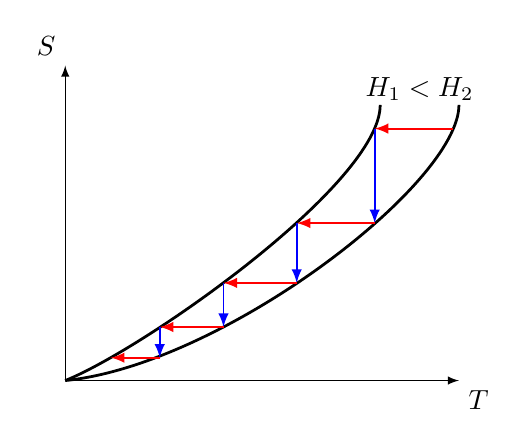
\begin{tikzpicture}
       \draw[-latex] (0,0) -- (5,0) node[below right] {$T$};
       \draw[-latex] (0,0) -- (0,4) node[above left] {$S$};
       \draw[line width=1pt] (0,0) .. controls (1,0.4) and (4,2.5) .. (4,3.5);
       \draw[line width=1pt] (0,0) .. controls (2,0.2) and (5,2.5) .. (5,3.5);
       \draw[-latex,line width=0.7pt,red] (4.92,3.2) -- (3.93,3.2);
       \draw[-latex,line width=0.7pt,blue] (3.93,3.2) -- (3.93,2);
       \draw[-latex,line width=0.7pt,red] (3.93,2) -- (2.94,2);
       \draw[-latex,line width=0.7pt,blue] (2.94,2) -- (2.94,1.24);
       \draw[-latex,line width=0.7pt,red] (2.94,1.24) -- (2.01,1.24);
       \draw[-latex,line width=0.7pt,blue] (2.01,1.24) -- (2.01,0.68);
       \draw[-latex,line width=0.7pt,red] (2.01,0.68) -- (1.2,0.68);
       \draw[-latex,line width=0.7pt,blue] (1.2,0.68) -- (1.2,0.29);
       \draw[-latex,line width=0.7pt,red] (1.2,0.29) -- (0.58,0.29);
       \node at (4.5,3.7) {$H_1 < H_2$};
       \end{tikzpicture}
       \caption{Az adiabatikus lemágnesezés folyamata. A piros lépésekben történik az adiabatikus lemágnesezés, a kék lépésekben pedig az izotermikus mágnesezés.}\label{fig:B03-adiablemag}
     \end{figure}
   \end{enumerate}
   